\section{Data} \label{sec:data}


\subsection{Dataset Analysis} \label{subsec:dataset}
When looking for datasets of film reviews, we wanted reviews that were linked to the film there were written for, preferrably also with a short summary of the film's plot.
What we found was mostly datasets that were intended for classification and a therefore positive/negative flag but no connection to the film.
Other datasets had too many information about the film, like the dataset that we ended up with \cite{dataset}, which included several information for all films on letterboxd.
These information are \texttt{url}, \texttt{title}, \texttt{year}, \texttt{directors}, \texttt{genres}, \texttt{cast}, \texttt{synopsis}, \texttt{rating}, \texttt{poster\_url}, and a maximum of 10 \texttt{reviews} each consisting of \texttt{username}, \texttt{review\_text}, and \texttt{likes}.
Of these we only need \texttt{title} and \texttt{year} to identify the film, the \texttt{synopsis} for context about the content of the film, and the \texttt{review\_text}s.
\\
Next, we analyzed this data which contains out of 847209 films and 2156477 reviews.
However, all these reviews were only linked to 366600 (43.27\%) of the films.
Of these films, 349753 (95.4\%) have a synopsis (of at least length 1) and the mean length is $\mu=44.8$ words.
Looking at the reviews, we see that besides many very short reviews, there are also many very long reviews, resulting in a mean length of $\mu=191.3$ words with a standard deviation of $\sigma=173.8$ words.
Using the lingua language detector \cite{lingua}, we found that 73.83\% of the reviews are written in English.
Running PySpellChecker \cite{PySpellChecker} on all reviews showed that 33.58\% of them have 0\% detected misspellings, and 52.76\% have less than 6\% detected misspellings.
With the EmojiPython package \cite{EmojiPython}, we counted the number of emojis per review and found that 96.08\% of all reviews have no emojis at all.
We used unicodedata \cite{unicodedata} to find both the number of non-latin characters per review (97\% of all reviews have no non-latin characterss at all) and the number of weird characters (So/Sm/Mn/Cf/Co) per review (93.88\% of all reviews have no weird characters at all).
The analysis results are visualized in Figure \ref{dataset_analysis}.
\\
\centerline{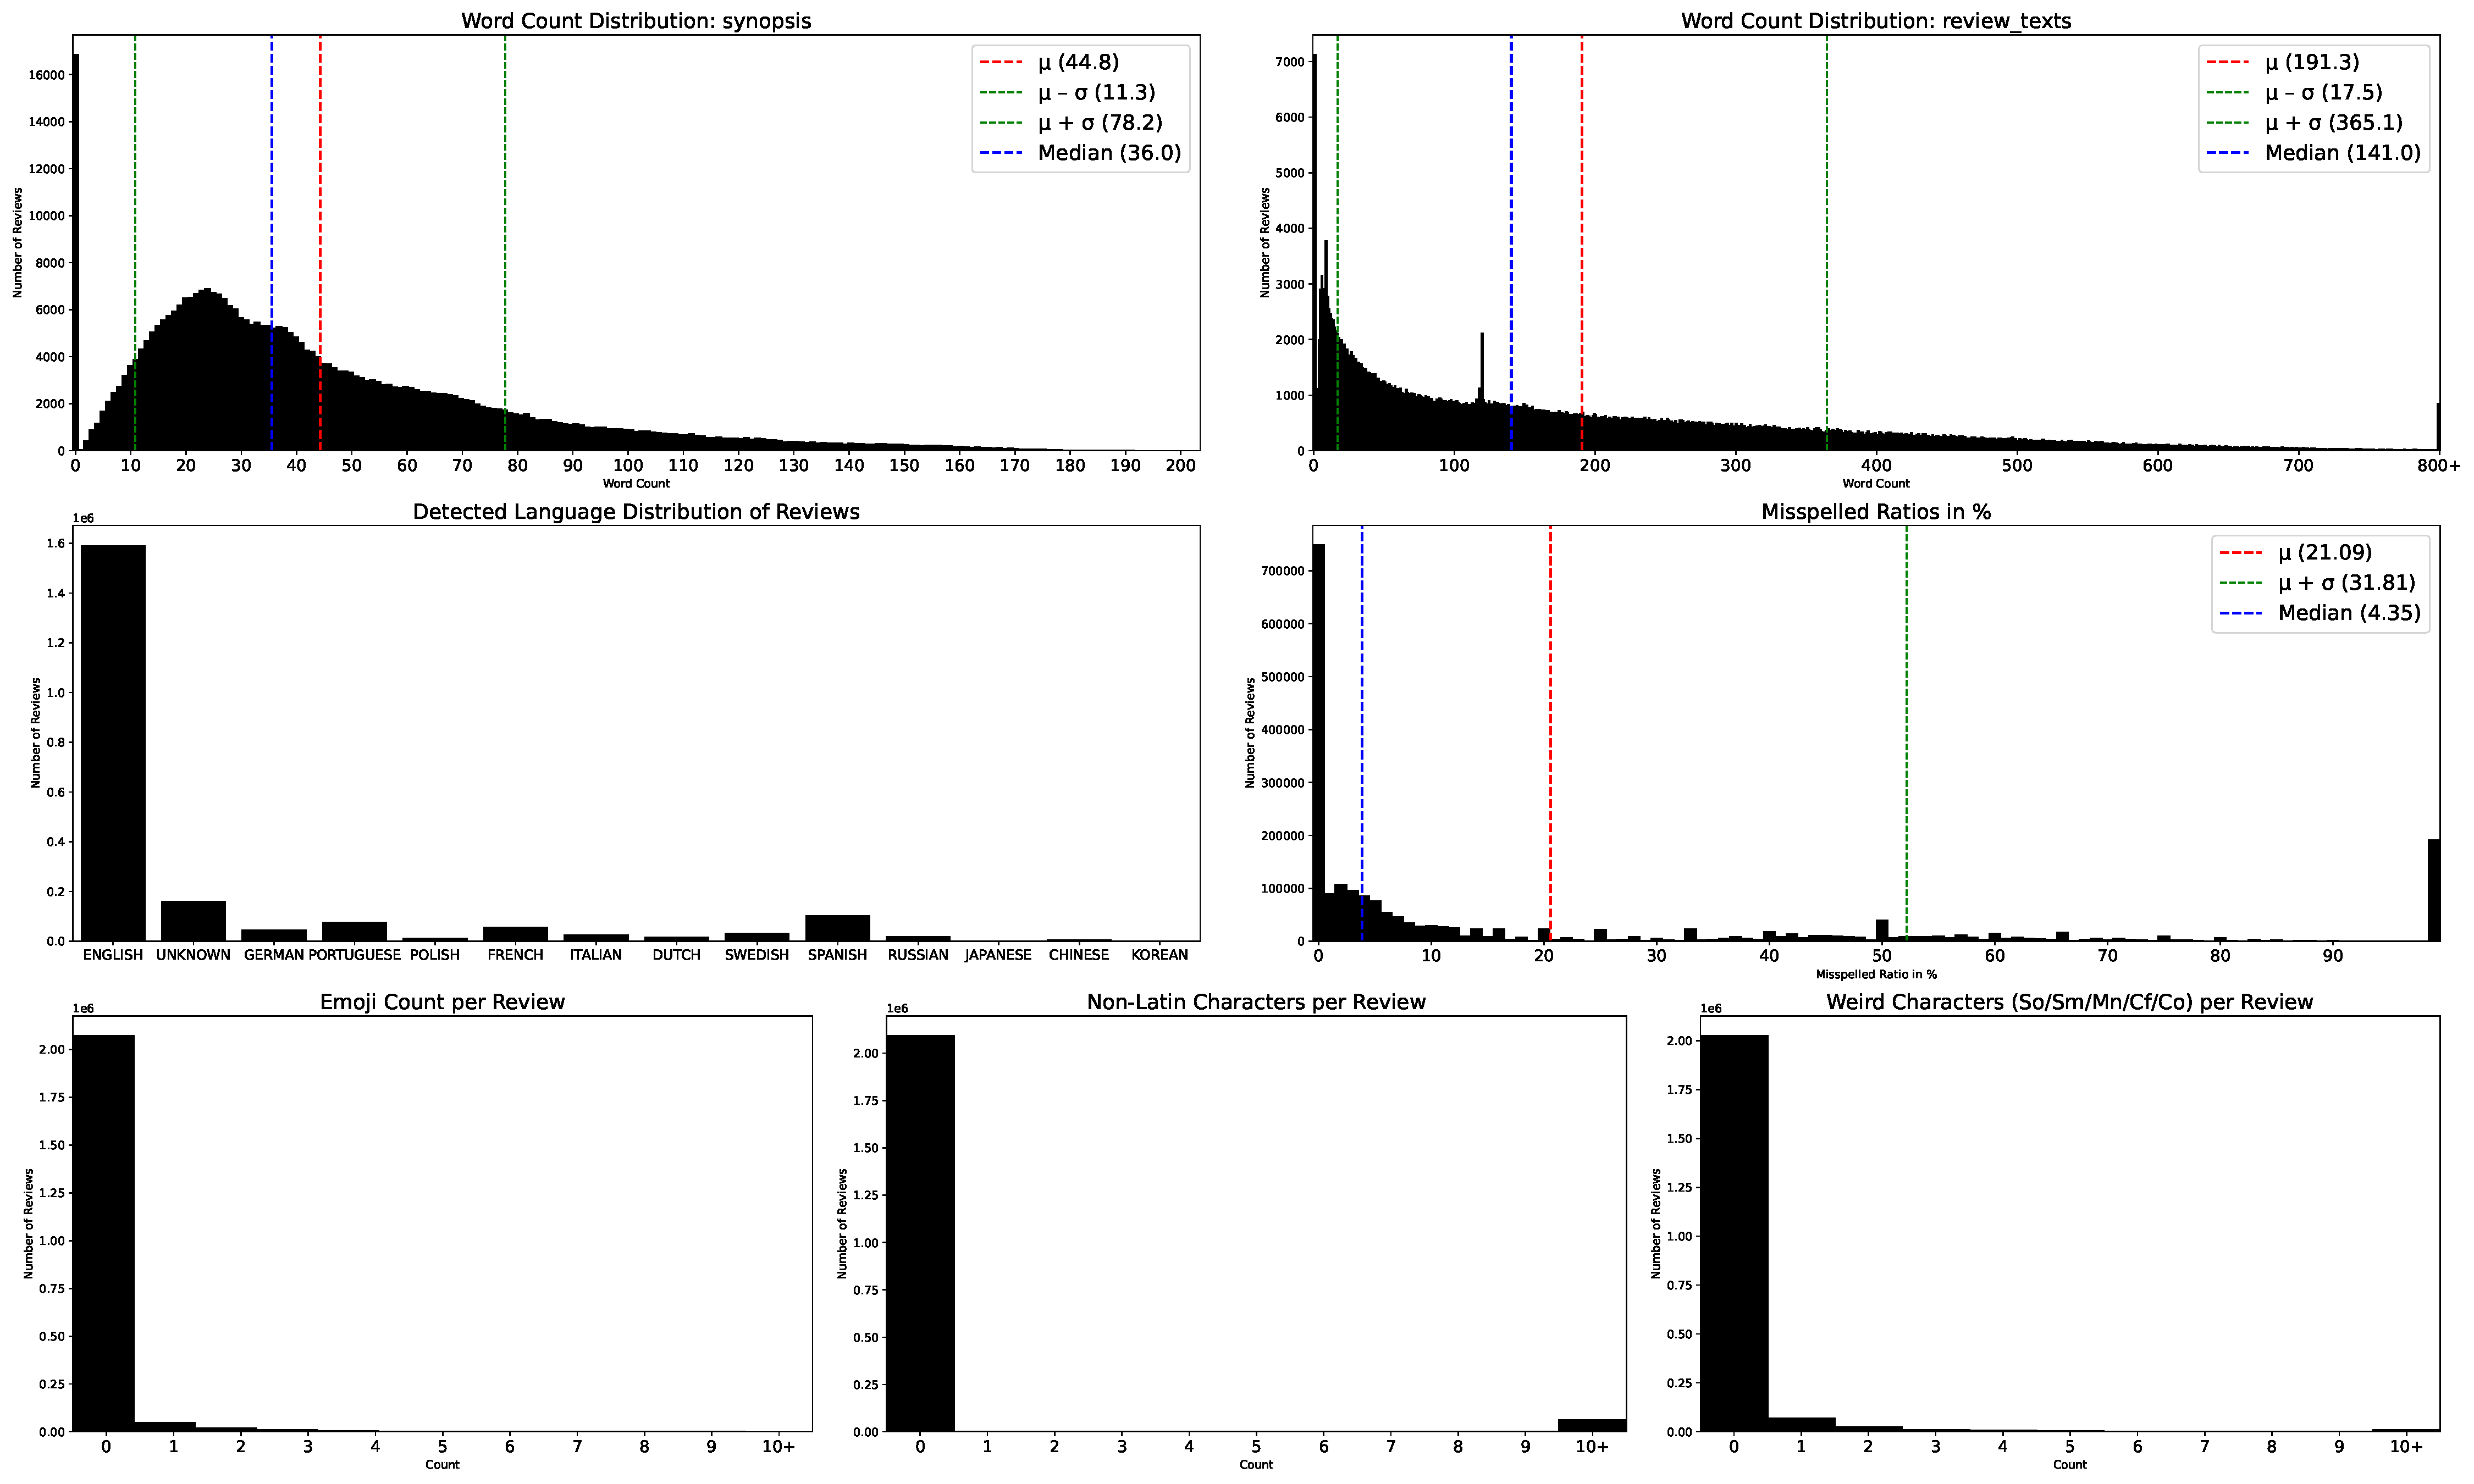
\includegraphics[scale=0.25]{images/dataset_analysis.pdf}} \label{dataset_analysis}


\subsection{Preprocessing} \label{subsec:preprocessing}
The preprocessing pipeline contains five stages which are depicted in Figure \ref{data_pipeline}.
The stages are the pre-filter, plots from OMDb, the mid-filter, review editing with LLM, and the post-filter.
While the three filter stages are used to remove reviews or entire films and therefore skrink the dataset, the other two stages expand it by adding information to the synopses and reviews.
\\
\centerline{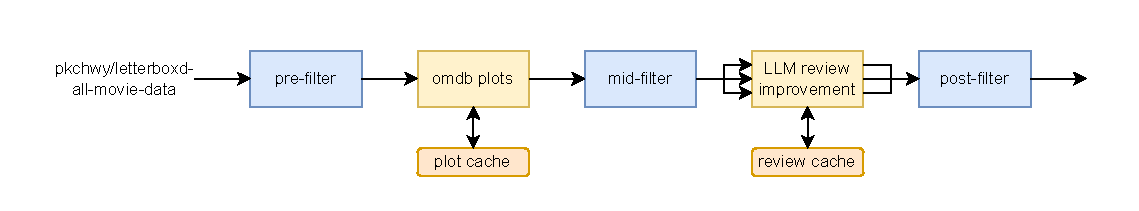
\includegraphics[scale=0.95]{images/data_pipeline.pdf}} \label{data_pipeline}


\subsubsection*{Pre-filter}
As a first step, the pre-filter removes duplicate reviews as these are often mistakes from the scraping process.
We also filtered out bad patterns that we found in many reviews like ``this review may contain spoilers'' (a letterboxd feature that hides a review with spoilers) or ``english version below'' (multi-language review, we would need only the english part).
What we also found often in the data were excessive repetitions of characters to express emotions.
For LM training these irregular patterns are not helpful and so we filter out any review were a single character is repeated more than 15 time in a row.
Then, based on the results of our dataset analysis, the pre-filter filters out reviews that
\begin{itemize}
  \setlength{\topsep}{0pt}
  \setlength{\itemsep}{0pt}
  \setlength{\parskip}{0pt}
  \item are shorter than 13 words
  \item are longer than 145 words
  \item include at least one emoji
  \item include more than 10 weird characters
  \item include any non-Latin characters
  \item are detected not to be written in English
  \item have more than 5\% of its words be detected as misspelled
\end{itemize}
Since reviews are already removed once they do not meet one of these criteria and checking the criteria takes varying amounts of time, the order in which these checks are conducted is important.
Specifically the spellcheck and language detection takes long, which is why they are run last.
\\
The pre-filter reduces the dataset from 847209 films and 2156477 reviews down to 239330 (28.25\%) films and 728258 (33.77\%) reviews.


\subsubsection*{Plots from OMDb}
In our analysis of the data, we realized that the synopsis is often too short.
In search for an alternative, we found the Open Movie Database (OMDb) API \cite{omdb-api}.
Access was granted after donating to the project via patreon \cite{omdb-api-patreon}.
The API allowed to search for films based on their name and year of creation and returned information about it like the \texttt{plot}, its \texttt{IMDb ID}, the \texttt{runtime}, \texttt{metascore}, \texttt{IMDb rating}, \texttt{IMDb votes}, and its \texttt{type}.
We saved these information for each film that we could find, and used some of them in the next stage for filtering.
Since the API allowed only for a limited number of requests per day, it was important to cache the results for the already queried films.


\subsubsection*{Mid-filter}
The mid-filter is mainly used to decide between the newly added plot from OMDb and the synopsis that was already included in the dataset:
If there is an OMDb plot for the film, it is almost always kept.  
Only when the synopsis is longer than the OMDb plot and the start the same, the synopsis is chosen.
If there is neither an OMDb plot nor a synopsis, the film is removed from the dataset.
\\
After this, we once again look at the length of the resulting synopsis/plot and remove films where this length is shorter than 20 words.
Furthermore, we use the additional metadata that we got from OMDb to remove small films that have less than 100 IMDb votes as reviews are unlikely to be good when the film has not gotten much attention overall. 
\\
All in all, the mid-filter reduces the dataset from 239330 films and 728258 reviews down to 236414 (98,78\%) films and 723885 (99.4\%) reviews.


\subsubsection*{Review Editing with LLM}
For better training on the user reviews, we decided to edit them using an LLM.
We wanted small rewrites that mostly fix the grammar, sentence structure, spelling, and spacing errors. % Beispiele? auch vielleicht sagen, dass wir das als Problem gefunden haben?
Since this is not a complicated task, a rather small language models should suffice.
Because we wanted to rewrite all of our remaining reviews, we needed the LLM to output many tokens quickly.  
We therefore decided to run a small language model, specifically Llama-3.2-1B-instruct with Q4\_K\_S quantization, locally via LM Studio.
% mehr zu Prompt & Rauswurf von DISCARD Reviews (wurden dadurch ja auch nochmal weniger)
As this is still time-intensive for many reviews, we split the dataset into equal parts and let the LLM run in parallel on multiple PCs for a speedup.
Similar to the plot fetching from OMDb, we also implemented a cache here that saves already rewritten reviews to save time and computation power in case of crashes.

\paragraph{Batch Processing Approach}
To further speedup the LLM processing, we tried a batch processing approach where we gave the LLM not just all reviews per film but multiple films and their reviews at once.
By doing so, the LLM would need to process the instructions only once and could use all computational resources for the text generation.
However, this batch processing failed with small 1B models, which could not process that big of an input and always returned DISCARD instead of the rewritten review.


\subsubsection*{Post-filter}
Since the LLM modified the reviews we found it helpful to run our pre-filter over them again.
The post-filter is essentially a modified pre-filter that allows for both longer and shorter reviews as 
The rest of the filter criteria are the same as in the pre-filter.
That way the post-filter reduces the dataset from 236414 films and 560627 reviews down to 212944 (90.07\%) films and 533625 (95.18\%) reviews.



\subsection{Tokenization} \label{subsec:tokenization}
